%%%%%%%%%%%%%%%%%%%%%%%%%%%%%%%%%%%%%%%%%%%%%%%%%%%%%%%%%%%%%%%%%%%%%%%%%%%%
\documentclass[a4j]{jarticle}

\usepackage{comment}
\usepackage{jsaisig}
\usepackage{algorithm,algorithmicx}
\usepackage{algpseudocode}
\usepackage[dvipdfmx]{graphicx}
%%%%%%%%%%%%%%%%%%%%%%%%%%%%%%%%%%%%%%%%%%%%%%%%%%%%%%%%%%%%%%%%%%%%%%%%%%%

\newcommand\todo[1]{@TODO[#1]}


\begin{document}
% 和文タイトル
\title{避難シミュレーションにおけるSNS上の情報伝達の効果について}

% 英文タイトル
\etitle{Effect of SNS communication in evacuation simulation} 

% 著者名: 
%	・各著者を\quad(全角空白)区切りで列挙
% 	・著者名の直後に\afil{所属番号}を追加→所属番号を上付で出力(\textsuperscript{所属番号}と同じ)
% 	 複数機関へ所属している場合は番号をカンマ区切りで列挙(下記著者2参照)
%  ・Corresponding Authorについては所属の後に\thanksを続け,連絡先を記入
%	・英文著者はカンマ区切りで列挙
\author{丹羽 俊徳\afil{1}%
 	\thanks{%
    連絡先: 名城大学 理工学部 情報工学科 \newline%
    〒468-8502 名古屋市天白区塩釜口1-501 \newline%
  	 E-mail: {e0930064@ccalumni.meijo-u.ac.jp}%
  }\quad%
 	岡谷 賢\afil{1} \quad 高橋 友一\afil{1}\\
  Toshinori Niwa\afil{1} \quad Masaru Okaya\afil{1} \quad Tomoichi Takahashi\afil{1}
}

% 所属
\affiliation{%
 	\afil{1} 名城大学 理工学部 情報工学科\\
  \afil{1} Meijo University, Department of Information Engineering
}

\abstract{%
During an emergency, information on the emergency is important to egress safely from buildings and to conduct rescue operations quickly.
Nowadays, almost everyone has mobile phones and they communicate each other using social network (SNS).
In this paper, we propose three types of communication model: broadcast, face to face (word of mouth), and SNS and demonstrate differences of evacuation effects.
}

\maketitle
\thispagestyle{empty}
%%%%%%%%%%%%%%%%%%%%%%%%%%%%%%%%%%%%%%


\section{はじめに}\label{sec:introduction}
災害時に正しい情報を適切に周知する事の重要性は言うまでもない\cite{tokuda:2011}。
災害時の救助活動や災害後の支援活動にと広くIT技術が使用されている\cite{COMMUNICATIONS}。
さらに、2001年のWTCや2011年の東日本大震災では、避難放送がいつ、どのようになされたか、その放送を聞いて人はどう行動したかについての報告がある\cite{NIST}\cite{muramoto:2012}。
同じ建物構造、同程度の人が避難したWTC1、WTC2からの異なる避難状況をシミュレーションするために、報告書の指摘内容や、人の心理状態に注目した、エージェントベースの避難シミュレーションも発表されている\cite{Nuria07}\cite{aamas11jason}\cite{okaya:2010}。

災害の発生、避難情報を伝える手段として、メディアや防災報道による一斉放送、電話などによる個人的な情報伝搬がある。
人が情報を受け取った直後や、その災害が身近に迫っていない時は、内容の確認をしたり身内の安否確認などをする事が報告されている。

その様な行動は50数年前のアメリカ、デンバーの洪水の事例でも報告されている\cite{drabek}。
人の行動様式に関わるこれらの知見を、今後の防災計画に反映するにあたり情報伝達の方法は時代にあった形態でシミュレーションする必要がある。
近年では、ほとんどの人は携帯電話を所有し、スマートフォンを所有しており、多くの人がソーシャルネットワーク(SNS)を利用している。

本論文では、SNSによる情報伝達が避難状況に与える影響を示し、今後の防災計画への避難シミュレーションへの適用可能性を示す。



\section{過去の報告}\label{sec:related-works}

{ISO/TR 16738}では、火災発生時に人が避難するまでの時間経過を${T}_{warn}$、$T_{pre}$、$T_{trav}$などに分類している。
\begin{description}
\item[$T_{warn}$:]{
  異常を見聞きしたり非常放送を聞くなど災害が起きた事を認識する段階。
  地震のように災害を直接認識する状況や、火災のように最初はごく一部の人しか異常を認識せず、少しずつ情報が広がって行く状況が考えられる。
}
\item[$T_{pre}$:]{
  災害が起きた事を個人が認識してから避難を開始するまでの段階。
  避難するかを相談したり、他の人に避難を促すといった行動をとる事が指摘されている。
}
\item[$T_{trav}$:]{
  避難を開始してから避難を終えるまでの段階。
}
\end{description}

表\ref{disaster-situation}に東日本大震災時の津波に対する時間の流れを示す。
津波が到達する約45分前には津波が到達することが分かっていた。
この45分間は、14:46から14:49までの$T_{warn}$と14:49から15:15までの$T_{evac}$の2段階に分けられる。
東日本大震災の報告書では、40\%の人しか非常放送を聞いていないことが報告された。
非常放送を聞いた人のうち、避難の必要性を感じた(即時避難)に対し、その他の人は雑音や混乱により避難の必要性を感じなかった(用事後避難、切迫避難)。
避難中にも、避難者同士がコミュニケーションをとり、行動を変更するといったことが報告されている\cite{muramoto:2012}。

図\ref{fig:wtc-comparison}はWTCのタワー1とタワー2の生存者がいつまで建物内にいたかの推移を示す。
同様な構造で同程度の人がいた状況での避難者の行動の相違を説明するには、人の行動パターンの相違に言及したシミュレーションが必要な事を示している。

\begin{table}[h]
\small
\centering
\caption{東日本大震災時の津波に対する時間の流れ}
\label{disaster-situation}
\begin{tabular}{|c||l|}\hline
Time
& Events \\ \hline
14:46 & Emergency earthquake alert system \\
      & Earthquake bulletins broadcasted.\\
      & The earthquake had \\
      & a moment magnitude of 9. \\
      & It continued for about 6 minutes.\\
14:49 & Tsunami warnings were issued:\\
      & ``A big tsunami will hit at around 15:10.''\\
15:15& Aftershocks occurred.\\
15:00-15:25& An initial, relatively small, tsunami struck.\\
15:25-15:40& A much larger tsunami arrived.\\ \hline
\end{tabular}
\end{table}

\begin{figure}[h]
\centering
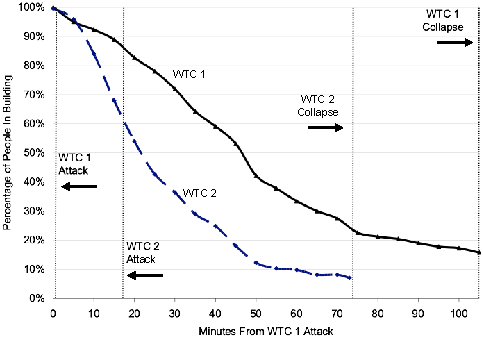
\includegraphics[width=\linewidth]{fig/wtc-comparison.pdf}
\caption{WTC1とWTC2における生存者が建物から避難した時間推移\cite{NIST}}
\label{fig:wtc-comparison}
\end{figure}


\begin{comment}
\begin{table}[h]
\begin{tabular}{|l||c|c|}\hline
reaction types           & $T_{warn}$  & $T_{pre}$ \\ \hline \hline
instant-evacuation       &  & 0 \\
evacuation-after-tasks   &  & minutes \\
                         &  & (Affiar task \\
                         &  & or seek information) \\
emergency-evacuation     &  & $\infty$(Affiar task) \\ \hline
\end{tabular}
\end{table}
\end{comment}


図\ref{fig:evac-model}は非常時発生から関連の人へ伝搬と避難対象者の行動モデルを示す。
人は火災報知器などの機器や発見者などからの情報をもとに、火災などの異常が発生した事を知る、
防災担当者は、非常時発生を知った段階で所定のマニュアルに従い発生と避難誘導報を行う。
個々の人は情報を知った後、その人の経験、訓練や人間関係など種々の要因に基づき、自分の判断で行動する。
エージェントベースシミュレーションは、その状況を表現する事がでる。
図では、BDIモデルで避難、確認、通報などの行動をするモデルを示している。
\begin{figure}[h]
\centering
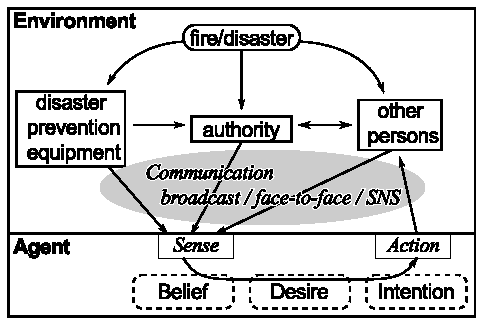
\includegraphics{fig/info-model.pdf}
\caption{情報伝達モデル。図中の矢印は情報伝達を示す。}
\label{fig:evac-model}
\end{figure}



\begin{comment}
\begin{figure}[h]
\centering
\begin{tabular}{c}
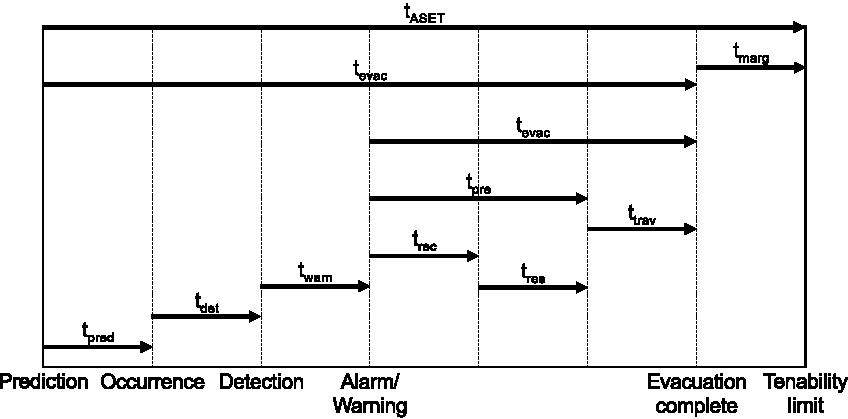
\includegraphics[clip,width=0.9\columnwidth]{fig/iso.pdf}
\end{tabular}
\caption{ISO/TR 16738}
\label{fig:iso}
\end{figure}
\end{comment}





%\cite{abbas:13}




\section{情報伝達と避難行動}\label{sec:sns-communication}

\subsection{情報源と情報手段}
同じ情報を受けても、人の行動パターンは様々である。
シャノンは情報通信をモデル化し、通信の問題を3段階に分類した\cite{shanon}。
\begin{description}
\item[段階A] {どのようにして、通信の記号を正確に伝送できるか(技術的問題)。}
\item[段階B] {どのようにして、伝送された記号が、伝えたい意味を正確に伝えるか(意味論的問題)。}
\item[段階C] {どのようにして、受け取られた意味が望む仕方で相手の行動に影響を与えるか(効果の問題)。}
\end{description}

この3段階A、B、Cは、非常時での通信で考えると、Aは混乱状況における騒音や環境条件による通信品質、
Bは災害が起きた事実と避難の必要性が間違いなく伝わる事、
Cは防災本部から市民への避難誘導放送であれば、安全な場所への移動が完了する事、家族間の安否確認であれば、お互いの安全を確認し、次の行動に結びつく情報を交換する事になる。


\begin{table}[h]
\centering
\caption{Communication methods}
\label{tab:communication-methods}
\begin{tabular}{|l||c|c|c|}\hline
          & broadcast & face-to-face & SNS \\ \hline\hline
range     & entire building & surrounding & no range \\ \hline
number    & large & small & middle \\ \hline
trust     & low & middle & high \\ \hline
          &\multicolumn{3}{l|}{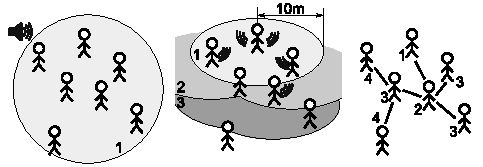
\includegraphics[width=6.7cm]{fig/trans-model.pdf}}\\\hline
\end{tabular}
\end{table}

%\begin{figure}[h]
%\centering
%\begin{tabular}{lcr}
%(a) broadcast ~~~& (b) face-to-face & ~~~(c) SNS\\
%\end{tabular}
%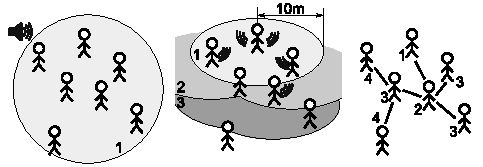
\includegraphics{fig/trans-model.pdf}
%\caption{避難情報の3種類の伝達手段}
%\end{figure}



\subsection{情報源の違いと信頼性}
東日本大震災や海外の災害においても、何度も行っても、避難する人の割合が100\%にならない事が報告されている。
そして、電話で情報を確認しようとしたが、話し中でつながらずに、結局何もしない報告もある。
人は、情報源によって同じ内容でも、信頼する/しない度合い(信頼性)が異なる。
表\ref{tab:communication-methods}に3つの通信形態の特徴をあげる。




\section{実験プラットフォーム}
\subsection{システム構成}
プロトタイプシステムは、RCRSをベースに構築した。
図\ref{fig:system-architecture}に、エージェントベースの避難シミュレーションシステムの構成を示す。
エージェントモジュール、環境モジュール、群衆シミュレーションモジュールからなる。
\begin{description}
\item[環境モジュール]{
  シミュレーションを行う場所の3D地図情報、エージェントモジュール間の通信管理を行う。
}
\item[エージェントモジュール]{
  エージェント一人一人の意思決定を行う。
  ステップ単位時間毎に、環境モジュールから受け取った情報を元に行動を決定する。
  BDIモデルを用いエージェントの動きを表現する。
}
\item[群衆シミュレーションモジュール]{
  エージェントの行き先情報に基づき通路などにおけるエージェントの歩行や混雑を粒子モデルに基づき計算する。
}
\end{description}

\subsection{エージェントの行動と通信コマンド}
エージェントは各ステップ($\Delta T$)毎に見聞きするデータを基に、自分の希望にあった行動を取る。
避難放送を聞いた後に指示に従って避難する今回のシミュレーションでは、図3に示す3種類のシナリオに対するアクションを実行する。

\begin{algorithm}
\caption{エージェントの行動($\Delta T$)}
\begin{algorithmic}[1]
  \If{避難情報を聞いた}
  \State {確率$p$で {\bfseries action}を実行}
  \EndIf
\end{algorithmic}
\end{algorithm}
{\bfseries action}として、後述するシナリオに対応して、
\begin{description}
 \item[action 1] 一番近い出口へ逃げる。
 \item[action 2] 一番近い出口へ逃げる。周囲のエージェントに避難情報を話す。
 \item[action 3] 一番近い出口へ逃げる。友人関係にあるエージェント全員に、一度だけ避難情報を伝える。
\end{description}
ここで確率$p$は段階Cにおいてエージェント内で情報を聞き、それを信じて行動に移す確率を表わす。

\begin{table}[h]
\centering
\caption{エージェントのコマンド}
\begin{tabular}[tb]{|c|c|c|}\hline
コマンド名 & コマンドの意味 & 具体例 \\ \hline \hline
\shortstack{say\\\vspace{3mm}} & \shortstack{周囲の人に\\ 情報を伝える} & \shortstack{避難情報を\\周りに伝える} \\
\hline
\shortstack{move\\\vspace{3mm}} & \shortstack{移動する\\\vspace{3mm}} &\shortstack{避難情報に\\基づいて逃げる} \\ \hline
\end{tabular}
\end{table}

\begin{figure}[h]
\centering
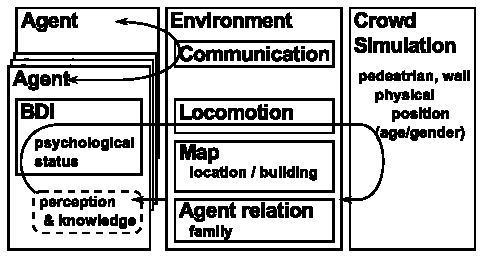
\includegraphics{./fig/system-architecture.pdf}
\caption{避難シミュレーションのシステム構成}
\label{fig:system-architecture}
\end{figure}


\section{実験}


\subsection{実験場所}
ユニモール(名古屋駅周辺の地下街)は長さ300m強のショッピングモールで、地下鉄の駅につながっている(図\ref{fig:unimall})。
周辺ビル、地上につながる出口が上下に14箇所ある。

\subsection{避難シナリオ}
3種類の情報伝達方法に対し、以下の3シナリオについてシミュレーションを行った。
\begin{figure}[h]
  \centering
  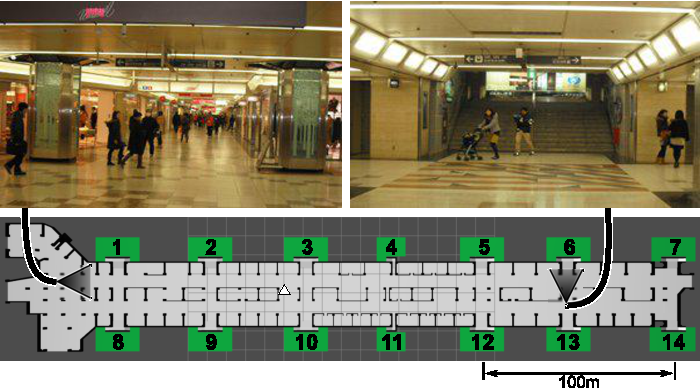
\includegraphics[width=\linewidth]{fig/unimall.pdf}
  \caption{ユニモール(名古屋駅周辺の地下街)、$\triangle$はシナリオ2、3におい
 て最初に情報を聞くエージェントの位置}
  \label{fig:unimall}
\end{figure}

\begin{description}
\item[Scenario 1]{%
  非常放送で一斉にすべての人に避難誘導を行う。
}
\item[Scenario 2]{%
  非常放送機器が故障した想定で、口答で避難誘導する。
  発話者から10m以内にいる人は内容を聞く事ができる。
}
\item[Scenario 3]{%
  避難者どうしがSNSでコミュニケーションをとった場合の避難。
  スタンフォード大学が提供している友人関係情報を元に、SNSにより通信する相手を決定する。
}
\end{description}


シナリオ1(一斉放送)では{\bfseries action 1}を、
シナリオ2(face to face)では{\bfseries action 2}を、
シナリオ3(SNS)では{\bfseries action 3}を用いた。
又、図\ref{fig:unimall}において、$\triangle$で示す場所にいるエージェントに対して最初のステップで情報が周知される。

避難情報の伝達手段の相違による3つのシナリオを実験した。シナリオ1、2、3と
も4039名のエージェントを配置し、シナリオ3ではデータに従ってエージェ
ント間のリンクを持っている。この4039名のエージェントはソーシャルネットワー
クを利用している大学生のデータである\cite{stanford-sns}。シナリオ3におけ
るエージェントの一次接続ノードの数の分布を図\ref{fig:friends-graph}に示
した。一次接続ノードの数は100未満が最も多い。一次接続ノードの数の最大は
1045人、最小は1人である。


\begin{figure}[t]
  \centering
  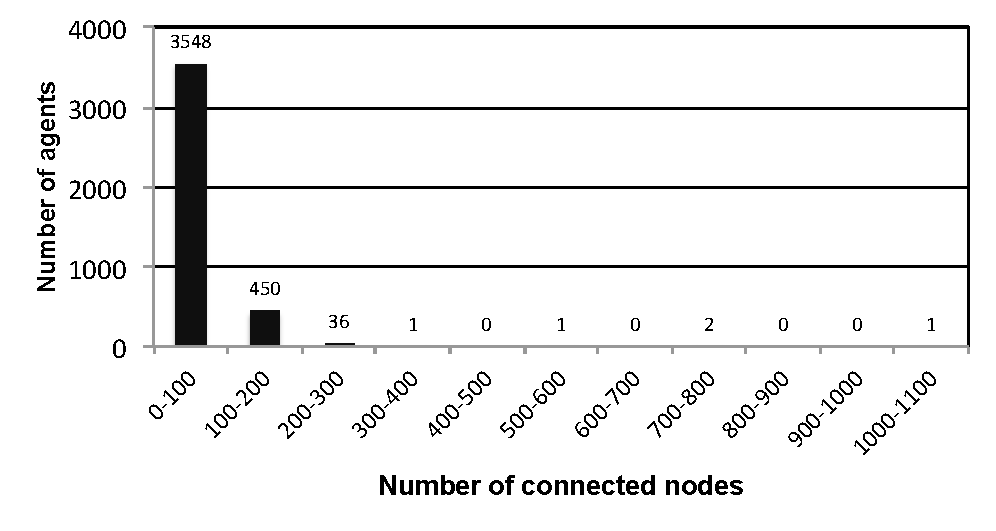
\includegraphics[width=\linewidth]{fig/number-of-friends.pdf}
\caption{エージェントの一次接続ノードの人数の分布、横軸は一次接続ノードの人数の範囲、縦軸はその範囲の一次接続ノードを持つエージェ
 ントの人数}
  \label{fig:friends-graph}
\end{figure}


\subsection{実験結果}
\subsubsection{即時避難の場合}
情報を聞いて即時に行動した($p=100\%$)シミュレーションは、理想の避難状況を
示している(図\ref{fig:exp-1}(a))。broadcastのシナリオ1では最初のステップで情報を知るエー
ジェントの割合(diffusion)は100\%で、出口に到着したエージェントの割合も
100\%に達している。

face to faceやSNSの初期状態は、図\ref{fig:unimall}の$\triangle$に示す位置に配置さ
れた1名のエージェントから情報が伝わるものとした。

% face to faceでは図\ref{fig:unimall-whole}に示すように
% 最終的に避難しなかった人が同じ場所に固まって存在している事がわかる。この
% 事は、図\ref{fig:unimall-whole}中の右端のエリアが出口から遠く、他の避難中エージェント
% が通らず避難情報が伝達されなかったためであると考えられる。
face to faceやSNSのシナリオを比較すると、情報伝達の速度に応じて避難率が上がっ
ていることがわかる。

\subsubsection{用事後避難}
$p=50\%$のときのシミュレーションを図\ref{fig:exp-1}(b)に示す。情報を聞い
た時に、すぐには避難せずに何らかの用事を済ませて避難する(用事後避難)人が
半数存在するという条件である。最初の一斉放送を一度しか聞く機会がないシナ
リオ1では避難率は50\%に留まる。face to faceでも避難率は約50\%(1973人)に留
まった。SNSでは最初に情報を聞いたときに避難行動に移らなかったとしても、そ
の後に他のエージェントからメッセージを聞く機会があるため、最終的に避難し
た人の人数が3869人と100\%近い避難率を達成している。

face to faceとSNSの避難した人数の結果の相違は、face to faceのエージェント
が移動しながら継続的に付近の人へ情報を伝達する一方、SNSではエージェントが
自分宛にメッセージがあったときだけ自分と友達関係にあるエージェントに情報
を伝達する事による。

\subsubsection{SNSでの情報の相違}
最初に情報を聞くエージェントの友人の多寡によって情報伝達効率は異なる。最
初に避難誘導を受けるエージェントの1次接続ノードの数が最大(1045)と最小(1)
のエージェントからシミュレーションした時の結果を図\ref{sns-ab}(a)と(b)に示す。避難開
始時には結果に差があるものの時刻が進むにつれて同じ傾向を示していることが
わかる。

\begin{figure}[h]
\centering
\begin{tabular}{c}
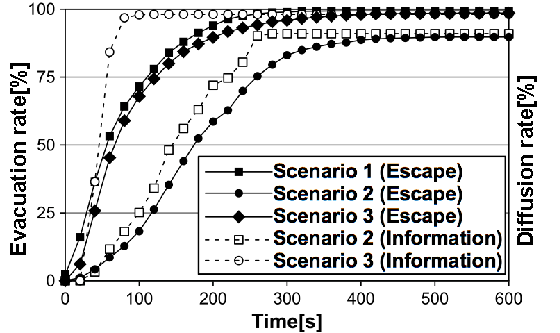
\includegraphics[height=\linewidth,angle=-90]{fig/p-100-plot-with-legend.pdf}\\
(a) $p=100\%$に対する結果\\
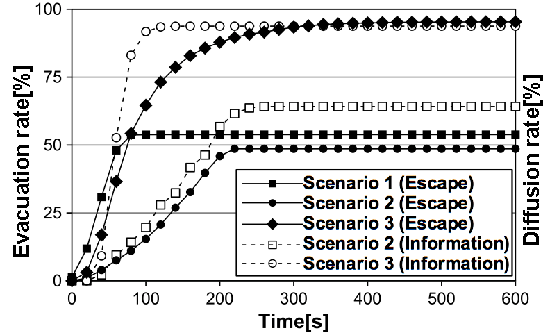
\includegraphics[height=\linewidth,angle=-90]{fig/p-50-plot-with-legend.pdf}\\
(b) $p=50\%$に対する結果\\
\end{tabular}
\caption{シナリオ(1)、(2)に対する避難状況と情報伝達}
\label{fig:exp-1}
\end{figure}

\begin{figure}[h]
\centering
\begin{tabular}{c}
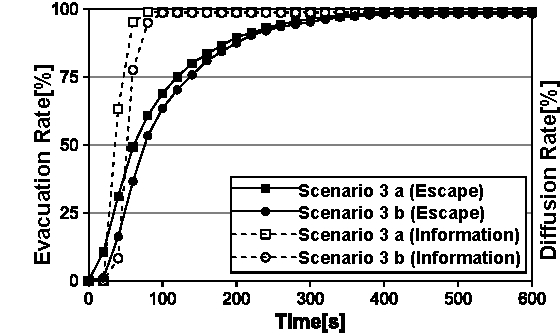
\includegraphics[width=\linewidth]{fig/p100-sns-20131009-1844.pdf}\\
(a) $p=100\%$に対する結果\\
\hspace{3mm}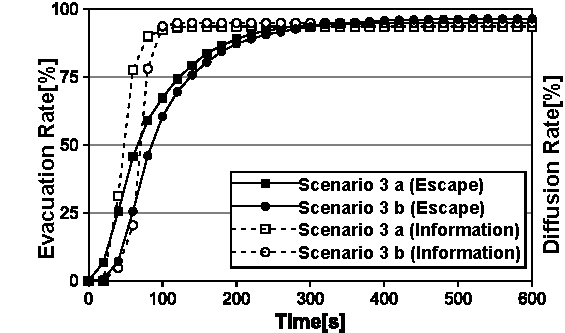
\includegraphics[width=\linewidth]{fig/p50-sns-20131009-1911.pdf}\\
(b) $p=50\%$に対する結果\\
\end{tabular}
\caption{SNSの構造の相違に対する避難状況と情報伝達((a)は図\ref{fig:exp-1}と同じ)}
\label{sns-ab}
\end{figure}

% \begin{figure}[t]
%   \centering
%   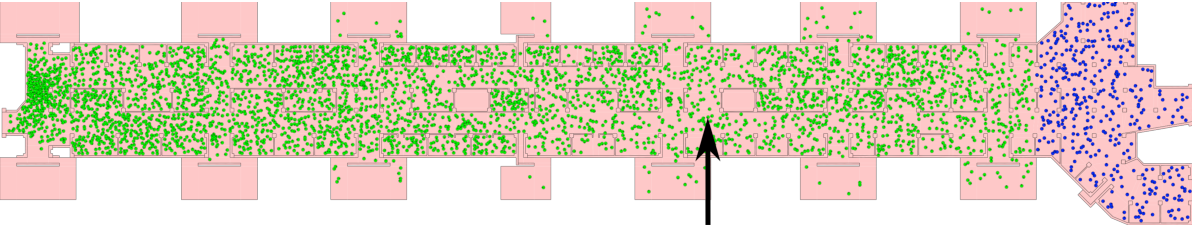
\includegraphics[width=\linewidth]{fig/whole_4.pdf}
%   \caption{Scenario 2 (face to face)のシナリオにおいて、最初に避難誘導を
%  受けた人(矢印)と、最終的に避難した人(緑色)と、最終的に避難しなかっ
%  た人(青色)}
%   \label{fig:unimall-whole}
% \end{figure}



\section{まとめ}
避難行動を考える上で、情報伝達を考える事は重要である。
従来の避難シミュレーションは避難誘導などの指示があった後、
建物などからの避難行動のシミュレーションを扱っていた。

本論文では非常事態が発生した情報を受け取った後、その情報が
周りの人に伝播していくモデルの一つとしてスマートフォンなど
によるソーシャルネットワークにおける情報伝達を取り上げ、
それが避難行動に及ぼす効果をシミュレーションした。






%%%%%%%%%%%%%%%%%%%%%%%%%%%%%%%%%%%%%%
%\section*{謝辞}
%%%%%%%%%%%%%%%%%%%%%%%%%%%%%%%%%%%%%%

\begin{thebibliography}{99}
%\small

\bibitem{abbas:13}
{{Abbas, A.}, {Muhammad, S.}}:
{Homophily, Popularity and Randomness: Modelling Growth of Online Social Network}
{\it AAMAS 2013} (2013)

\bibitem{fridman:13}
{{Fridman, N.}, {Kaminka, G.}, {Zilka, A.}}:
{The Impact of Culture on Crowd Dynamics: An Empirical Approach}
{\it AAMAS 2013} (2013)
\bibitem{:13}

{{Hui, C.}, {Goldberg, M.}, {Magdon-Ismail, M.}, {Wallace, W.}}:
{Simulating the Diffusion of Information: An Agent-Based Modeling Approach}
{\it AAMAS 2013} (2013)

\bibitem{muramoto:2012}
邑本 俊亮:
避難と情報
{\it 電子情報通信学会誌}, Vol.~95, No.~10, pp.~894--898 (2012)

\bibitem{tokuda:2011}
徳田 雄洋:
震災と情報?あのとき何が伝わったか
{\it 岩波書店}, (2011)

\bibitem{COMMUNICATIONS}
{Walle, B.}, {Turoff, B.}:
{Emergency Response Information Systems: EMERGING TRENDS AND TECHNOLOGIES}
{\it Association for Computing Machinery}, Vol.~50, No.~3, pp.~29--31 (2007)

\bibitem{Nuria07}
Nuria Pelechano and Ali Malkawi:
Comparison of crowd simulaton for building evacuation and an alternateive approach
{\it In Building Simulation 2007}, pp.~1514--1514 (2007)

\bibitem{aamas11jason}
Jason Tsai et al.:
{{ESCAPES} - Evacuation Simulation with Children, Authorities, Parents, Emotions, and Social comparison}
{\it AAMAS 2011}, (2011)

\bibitem{okaya:2010}
岡谷賢, 高橋友一:
人間関係を考慮したエージェントベースの避難シミュレーションフ レームワーク
{\it 電子情報通信学会誌}, Vol.~J94, No.~11, pp.~1855--1865 (2011)

\bibitem{drabek}
Drabek, T.:
The Human Side of Disaster, Second Edition
{\it CRS Press}, Vol.~95, No.~10 pp.~859--952 (2013)

\bibitem{stanford-sns}
Stanford University:
Social circles: Facebook
{http://snap.stanford.edu/data/egonets-Facebook.html}

\bibitem{NIST}
Averill, J.:
NISTncstar 1-7: Occupant behavior, egress, and emergency communication
(2005)

\bibitem{shanon}
クロード・E. シャノン, ワレン ウィーバー:
通信の数学的理論
{\it 筑摩書房} (2009)


\begin{comment}
\bibitem{}
First, A., Second, A.:
Homophily, Popularity and Randomness: Modelling Growth of Online Social Network
{\it Journal Name}, Vol.~xx, No.~x, pp.~xx--xx (2007)
\end{comment}




\end{thebibliography}

\end{document}